%============================================================
% MTH 112 Project - Other Trig Functions
% Updated 202504
%============================================================

\section{Other Trigonometric Functions} \label{section-other-trigonometric-functions}
In this section, we will find exact values of the trigonometric functions secant, cosecant, tangent, and cotangent of $\frac{\pi}{3}$, $\frac{\pi}{4}$, and $\frac{\pi}{6}$, use reference angles to evaluate the trigonometric functions secant, tangent, and cotangent, use properties of even and odd trigonometric functions, recognize and use fundamental identities, and evaluate trigonometric functions with a calculator.

\textbook{\href{https://openstax.org/books/algebra-and-trigonometry-2e/pages/7-4-the-other-trigonometric-functions}{7.4}}

\subsection*{Preparation Exercises} \label{preparation-exercises-section-other-trigonometric-functions}

Answer the following without using a calculator. These questions are intended to check the prerequisite skills needed to complete the rest of the lab.

\begin{myPrep}
	What did \say{CHOSHACAO} stand for back in Exercise \ref{CHOSHACAO} from Section \ref{section-right-triangle-trigonometry}?
\end{myPrep}
\vfill

\begin{myPrep}
	What is the value of $\sin\left(\frac{\pi}{3}\right)$?
\end{myPrep}
\vfill

\begin{myPrep}
	Find the value of $\cos\left(\frac{11\pi}{4}\right)$ using your memorized unit circle values and a reference angle.
\end{myPrep}
\vfill

\begin{myPrep}
	Find the value of $\sin\left(-\frac{2\pi}{3}\right)$ using your memorized unit circle values and a reference angle.
\end{myPrep}
\vfill

\begin{myPrep}
	Explain what makes a function an \say{odd function}? %ISSUE: reference odd and even functions from 111Z.
\end{myPrep}
\vfill

%======================================================
\newpage
%======================================================

\subsection*{Practice Exercises} \label{practice-exercises-section-other-trigonometric-functions}


\begin{myPractice}
	Find all six trigonometric function values given the coordinates of the point at an angle $\gamma$ on a unit circle.
	\begin{multicols}{2}
		\begin{center}
			\captionsetup{type=figure} \captionof{figure}{A point on a unit circle at an angle $\gamma$}
			\begin{tikzpicture}
				\begin{axis}[
					% framed,
					xmin=-1.2,xmax=1.2,
					ymin=-1.2,ymax=1.2,
			       	xtick={-1,1},
			       	ytick={-1,1},
			       	clip=false,
					]
						\draw 	(axis cs:0,0) circle [radius=1];
						\addplot[mark=*,color=first] coordinates{(-0.866,0.5)};
						\draw 	(-0.866,0.5) node[above left,color=first] {\scriptsize{$\left(-\frac{\sqrt{3}}{2},\frac{1}{2}\right)$}};
						\addplot[variable=\t, domain=0:150, samples=50, color=third]({.2*cos(t)}, {.2*sin(t)});
						\draw 	(0.1,0.1) node[above right,color=third] {$\gamma$};
						\draw   [color=fourth,very thick,mark=*](0,0)--(-0.866,0.5);
				\end{axis}
			\end{tikzpicture}\label{fig:exercise-other-trig-functions-from-point}
		\end{center}
		\columnbreak
		\begin{enumerate}
			\item $\sin(\gamma)$
			\vfill
			\item $\cos(\gamma)$
			\vfill
			\item $\csc(\gamma)$
			\vfill
			\item $\sec(\gamma)$
			\vfill
			\item $\tan(\gamma)$
			\vfill
			\item $\cot(\gamma)$
			\vfill
		\end{enumerate}
	\end{multicols}
\end{myPractice}

\begin{myPractice}
	Find all six trigonometric function values at the angle $\frac{\pi}{3}$ using your memorized values for the $\sin\left(\frac{\pi}{3}\right)$ and $\cos\left(\frac{\pi}{3}\right)$.
	\begin{enumerate}
		\begin{multicols}{2}
			\item $\sin\left(\frac{\pi}{3}\right)$
			\vspace{.5cm}
			\item $\cos\left(\frac{\pi}{3}\right)$
			\vspace{.5cm}
			\item $\csc\left(\frac{\pi}{3}\right)$
			\vfill
			\item $\sec\left(\frac{\pi}{3}\right)$
			\vspace{.5cm}
			\item $\tan\left(\frac{\pi}{3}\right)$
			\vspace{.5cm}
			\item $\cot\left(\frac{\pi}{3}\right)$
			\vfill
		\end{multicols}
	\end{enumerate}
\end{myPractice}

\begin{myPractice}
	Find the trigonometric function values given the right triangle with lengths shown in Figure \ref{fig:section-other-trig-functions-practice}.
	\begin{multicols}{2}
		\begin{center}
		\captionsetup{type=figure} \captionof{figure}{A right triangle}
			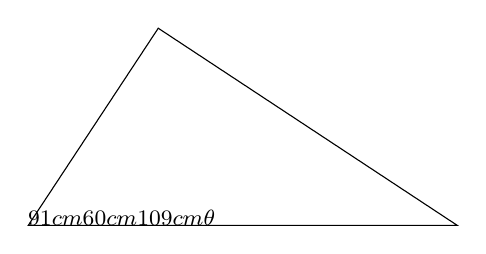
\begin{tikzpicture}[thin,scale=0.5]
				\coordinate (O) at (3.30275,5.00917);
				\coordinate (B) at (0,0);
				\coordinate (A) at (10.9,0);
				\draw (O)--(A)--(B)--cycle;
				\footnotesize
				\tkzLabelSegment[above=2pt,rotate=-atan(5.00917/7.5972)](O,A){$91\text{cm}$}
				\tkzLabelSegment[above=2pt,rotate=atan(5.00917/3.30275)](O,B){$60\text{cm}$}
				\tkzLabelSegment[below=2pt](A,B){$109\text{cm}$}
				\tkzMarkRightAngle[size=0.5](A,O,B)
				\tkzMarkAngle[size=0.8cm](A,B,O)
				\tkzLabelAngle[pos = 1,right](A,B,O){$\theta$}
			\end{tikzpicture}\label{fig:section-other-trig-functions-practice}
		\end{center}
		\columnbreak
		\begin{enumerate}
			\item $\sin(\theta)$
			\vspace{.5cm}
			\item $\csc(\theta)$
			\vspace{.5cm}
			\item $\sec(\theta)$
			\vspace{.5cm}
			\item $\cot(\theta)$
			\vspace{.5cm}
		\end{enumerate}
	\end{multicols}
\end{myPractice}

%======================================================
\newpage
%======================================================

\begin{myPractice}
	Fill in a table of all 6 trig values for the standard angles on the unit circle.
	\begin{center}
		\renewcommand{\arraystretch}{2} 
		\begin{tabular}{|| c | P{1.5cm} | P{1.5cm} | P{1.5cm} | P{1.5cm} | P{1.5cm} ||}
			\hline
			$\theta$ & $0$ & $\frac{5\pi}{6}$ & $\frac{\pi}{4}$ & $\frac{4\pi}{3}$ & $\frac{\pi}{2}$ \\
			\hline
			$\sin(\theta)$ & & & & &\\ 
			\hline
			$\cos(\theta)$ & & & & &\\ 
			\hline
			$\csc(\theta)$ & & & & &\\ 
			\hline
			$\sec(\theta)$ & & & & &\\ 
			\hline
			$\tan(\theta)$ & & & & &\\ 
			\hline
			$\cot(\theta)$ & & & & &\\ 
			\hline
		\end{tabular}
	\end{center}
\end{myPractice}

% \begin{myPractice}
% 	Fill in a table of all 6 trig values for the standard angles on the unit circle using knowledge of reference angles.
% 	\begin{center}
% 		\renewcommand{\arraystretch}{1.5} 
% 		\begin{tabular}{|| c | P{1cm} | P{1cm} | P{1cm} | P{1cm} | P{1cm} ||}
% 			\hline
% 			$\theta$ & $\pi$ & $\frac{5\pi}{6}$ & $\frac{7\pi}{4}$ & $\frac{4\pi}{3}$ & $\frac{3\pi}{2}$ \\
% 			\hline
% 			$\sin(\theta)$ & & & & &\\ 
% 			\hline
% 			$\cos(\theta)$ & & & & &\\ 
% 			\hline
% 			$\csc(\theta)$ & & & & &\\ 
% 			\hline
% 			$\sec(\theta)$ & & & & &\\ 
% 			\hline
% 			$\tan(\theta)$ & & & & &\\ 
% 			\hline
% 			$\cot(\theta)$ & & & & &\\ 
% 			\hline
% 		\end{tabular}
% 	\end{center}
% \end{myPractice}

\begin{myPractice}
	Use the fact that $\sin(x)$, $\tan(x)$, $\cot(x)$, and $\csc(x)$ are odd and $\cos(x)$ and $\sec(x)$ are even to fill in the following values.
	\begin{enumerate}
		\begin{multicols}{2}
			\item $\sin\left(-\frac{2\pi}{3}\right)$
			\vspace{2cm}
			\item $\tan\left(-\frac{2\pi}{3}\right)$
			\vspace{2cm}
			\item $\cot\left(-\frac{2\pi}{3}\right)$
			\item $\csc\left(-\frac{2\pi}{3}\right)$
			\vspace{2cm}
			\item $\cos\left(-\frac{2\pi}{3}\right)$
			\vspace{2cm}
			\item $\sec\left(-\frac{2\pi}{3}\right)$
		\end{multicols}
	\end{enumerate}
\end{myPractice}
\vfill

%======================================================
\newpage
%======================================================

\begin{myPractice}
	Find the other trigonometric values for the angle shown in each part.
	\begin{enumerate} 
		\item $\sec(\psi)=-\frac{7}{2}$ and $\frac{\pi}{2}\le\psi\le\pi$.
		\vfill
		\item $\cot(\zeta)=-\frac{6}{5}$ and $\frac{3\pi}{2}\le\zeta\le2\pi$.
		\vfill
	\end{enumerate}
\end{myPractice}

%======================================================
\newpage
%======================================================

\subsection*{Definitions} \label{def-other-trigonometric-functions}

\begin{multicols}{2}
	\begin{myDefinition}[{The \say{Other} Trigonometric Functions}]~\\[0.5mm]
		For a right triangle with with angle $\theta$, the \say{\textbf{other trigonometric functions}} can be found by the following definitions as in Figure \ref{fig:other-trig-functions}. Visit \href{http://tiny.cc/six-trig-functions}{this interactive Desmos graph} to see the six trigonometric lengths in action. \qrcode[height=1cm]{http://tiny.cc/six-trig-functions}
		\begin{itemize}
				\item $\tan(\theta)=\frac{\sin(\theta)}{\cos(\theta)}$
				\item $\cot(\theta)=\frac{\cos(\theta)}{\sin(\theta)}$
				\item $\sec(\theta)=\frac{1}{\cos(\theta)}$
				\item $\csc(\theta)=\frac{1}{\sin(\theta)}$
		\end{itemize}
	\end{myDefinition}

	\begin{center}
		\captionsetup{type=figure} \captionof{figure}{Other trigonometric function definitions}
		\begin{tikzpicture}
			\begin{axis}[
				framed,
				xmin=-1.1,xmax=1.8,
				ymin=-1.1,ymax=1.8,
		       	xtick={-1,1},
		       	ytick={-1,1},
				]
					\draw 	(axis cs:0,0) circle [radius=1];
					\addplot[mark=*,color=first] coordinates{(0.6,0.8)(0,0)(0.6,0)};
					\addplot[mark=*,color=first] coordinates{(1.67,0)(0,1.25)};
					\draw   [color=first, very thick](0,0)--(0.6,0.8);
					\draw 	(0.3,0.4) node[above,color=first,rotate=53.13] {\scriptsize{$r=1$}};
					\addplot[variable=\t, domain=0:atan(4/3), samples=50,very thin, color=third]({.2*cos(t)}, {.2*sin(t)});
					\draw 	(0.25,0.07) node[left,color=third] {\tiny$\theta$};
					\draw   [color=fourth,very thick](0,0)--(0.6,0);
					\draw 	[decorate, pen colour={fourth}, decoration = {calligraphic brace, mirror, amplitude=3pt}] (0,0)--(0.6,0) node[pos=0.5,below,color=fourth] {\scriptsize$\cos(\theta)$};
					\draw   [color=second, very thick](0.6,0)--(0.6,0.8);
					\draw 	(0.6,0.3) node[above,color=second,rotate=-90] {\scriptsize$\sin(\theta)$};
					\draw   [color=third, very thick](5/3,0)--(0.6,0.8);
					\draw 	[decorate, pen colour={third}, decoration = {calligraphic brace, amplitude=5pt, mirror}] (1.76,.1)--(0.7,0.9) node[pos=0.5,above,color=third,rotate=-36.87] {\scriptsize$\tan(\theta)$};
					\draw   [color=fourth, very thick](0.6,0.8)--(0,1.25);
					\draw 	[decorate, pen colour={fourth}, decoration = {calligraphic brace, amplitude=5pt, mirror}] (0.7,0.9)--(0.1,1.35) node[pos=0.5,above,color=fourth,rotate=-36.87] {\scriptsize$\cot(\theta)$};
					\draw   [color=fifth, very thick,dashed](5/3,0)--(0,0);
					\draw 	[decorate, pen colour={fifth}, decoration = {calligraphic brace, mirror, amplitude=5pt, aspect=0.4}] (0,-0.2) --  (1.67,-0.2) node[pos=0.4,below,color=fifth] {\scriptsize$\sec(\theta)$};
					\draw   [color=second, very thick](0,0)--(0,1.25);
					\draw 	[decorate, pen colour={second}, decoration = {calligraphic brace, amplitude=5pt}] (-0.1,0) --  (-0.1,1.25) node[pos=0.5,above,color=second,rotate=90] {\scriptsize$\csc(\theta)$};
			\end{axis}
		\end{tikzpicture}
		\label{fig:other-trig-functions}
	\end{center}
\end{multicols}

\vfill

\begin{multicols}{2}
	\begin{myDefinition}[{CHOSHACAO}]~\\[0.5mm]
		For a right triangle with hypotenuse $h$, and sides $x$, and $y$, as in Figure \ref{fig:other-trig-functions-CHOSHACAO}, tangent is still \say{opposite over adjacent}, as you saw in \hyperref[section-right-triangle-trigonometry]{the section about right-triangle trigonometry} and the \say{other trigonometric function values} can be found with \say{\textbf{CHOSHACAO}}. 
		\begin{itemize}
			\item $\tan(\theta)=\frac{y}{x}=\frac{\text{Opposite}}{\text{Adjacent}}$
			\item $\cot(\theta)=\frac{x}{y}=\frac{\text{Adjacent}}{\text{Opposite}}$
			\item $\sec(\theta)=\frac{h}{x}=\frac{\text{Hypotenuse}}{\text{Adjacent}}$
			\item $\csc(\theta)=\frac{h}{y}=\frac{\text{Hypotenuse}}{\text{Opposite}}$
		\end{itemize}
		\columnbreak

		\begin{center}
		\captionsetup{type=figure} \captionof{figure}{A right triangle}
			\begin{tikzpicture}[thin, scale=2]
				\coordinate (O) at (0,0);
				\coordinate (A) at (3,0);
				\coordinate (B) at (0,2);
				\draw (O)--(A)--(B)--cycle;
				\footnotesize
				\tkzLabelSegment[below=2pt](O,A){$x$\text{, Adjacent}}
				\tkzLabelSegment[above=2pt, rotate=90](O,B){$y$\text{, Opposite}}
				\tkzLabelSegment[above=2pt, rotate=-atan(2/3)](A,B){$h$\text{, Hypotenuse}}
				\tkzMarkRightAngle[size=0.5](A,O,B)
				\tkzMarkAngle[size=0.8cm](B,A,O)
				\tkzLabelAngle[pos = 0.6](B,A,O){\large$\theta$}
			\end{tikzpicture}
			\label{fig:other-trig-functions-CHOSHACAO}
		\end{center}
	\end{myDefinition}
\end{multicols}

\vfill

\begin{multicols}{2}
	\begin{myDefinition}[{Even and Odd Trigonometric Functions}]~\\[0.5mm]
		Recall that even functions are symmetrical about the $y$-axis, which makes 
		$f(x)=f(-x)$, and odd functions are symmetrical about the origin, which makes $-f(x)=f(-x)$. All of the trigonometric functions are either even or odd. Here's a list:
		\columnbreak
		\begin{itemize}
			\item $\sin(-x)=-\sin(x)$, so $\sin(x)$ is odd.
			\item $\tan(-x)=-\tan(x)$, so $\tan(x)$ is odd.
			\item $\cot(-x)=-\cot(x)$, so $\cot(x)$ is odd.
			\item $\csc(-x)=-\csc(x)$, so $\csc(x)$ is odd.
			\item $\cos(-x)=\cos(x)$, so $\cos(x)$ is even.
			\item $\sec(-x)=\sec(x)$, so $\sec(x)$ is even.
		\end{itemize}
	\end{myDefinition}
\end{multicols}

\vfill

\begin{multicols}{2}
	\begin{myDefinition}[{Other Pythagorean identities}]~\\[0.5mm]
		You already know that $\sin^2(\theta)+\cos^2(\theta)=1$, and that this is called the \textbf{Pythagorean Identity}. There are two other Pythagorean relationships which you can see Figure \ref{fig:other-pythag-identities}, which is a trimmed-down version of Figure \ref{fig:other-trig-functions}. 
		\begin{itemize}
			\item $\tan^2(\theta)+1=\sec^2(\theta)$
			\item $\cot^2(\theta)+1=\csc^2(\theta)$
		\end{itemize}
	\end{myDefinition}
	\columnbreak
	\begin{center}
		\captionsetup{type=figure} \captionof{figure}{Other Pythagorean Identities}
		\begin{tikzpicture}
			\begin{axis}[
				framed,
				xmin=-1.1,xmax=1.8,
				ymin=-1.1,ymax=1.8,
		       	xtick={-1,1},
		       	ytick={-1,1},
				]
					\draw 	(axis cs:0,0) circle [radius=1];
					\addplot[mark=*,color=first,mark size=1pt] coordinates{(0.6,0.8)(0,0)};
					\addplot[mark=*,color=first,mark size=1pt] coordinates{(1.67,0)(0,1.25)};

					\draw   [thin,color=fourth](0.7,0.725)--(0.622,0.621)--(0.522,0.696);
					\draw   [thin,color=second](0.5,0.875)--(0.422,0.771)--(0.522,0.696); %these are kludgy ways of getting right angle markers but the markrightangle command doesn't work within an axis environment.

					\draw   [color=first, very thick](0,0)--(0.6,0.8);
					\draw 	(0.3,0.4) node[above,color=first,rotate=53.13] {\footnotesize{$r=1$}};
					\addplot[variable=\t, domain=0:atan(4/3), samples=50,very thin, color=first]({.2*cos(t)}, {.2*sin(t)});
					\draw 	(0.15,0.1) node[right,color=first] {\footnotesize$\theta$};

					\draw   [color=fourth, very thick](5/3,0)--(0.6,0.8);
					\draw 	[decorate, pen colour={fourth}, decoration = {calligraphic brace, amplitude=5pt, mirror}] (1.76,.1)--(0.7,0.9) node[pos=0.5,above,color=fourth,rotate=-36.87] {\footnotesize$\tan(\theta)$};
					\draw   [color=fourth, very thick](5/3,0)--(0,0);
					\draw 	[decorate, pen colour={fourth}, decoration = {calligraphic brace, mirror, amplitude=5pt, aspect=0.4}] (0,-0.1) --  (1.67,-0.1) node[pos=0.4,below,color=fourth] {\footnotesize$\sec(\theta)$};

					\draw   [color=second, very thick](0.6,0.8)--(0,1.25);
					\draw 	[decorate, pen colour={second}, decoration = {calligraphic brace, amplitude=5pt, mirror}] (0.7,0.9)--(0.1,1.35) node[pos=0.5,above,color=second,rotate=-36.87] {\footnotesize$\cot(\theta)$};
					\draw   [color=second, very thick](0,0)--(0,1.25);
					\draw   [color=second, thin](0.6,0.8)--(0,1.25);
					\draw 	[decorate, pen colour={second}, decoration = {calligraphic brace, amplitude=5pt}] (-0.1,0) --  (-0.1,1.25) node[pos=0.5,above,color=second,rotate=90] {\footnotesize$\csc(\theta)$};
			\end{axis}
		\end{tikzpicture}
		\label{fig:other-pythag-identities}
	\end{center}
\end{multicols}

\vfill

\begin{multicols}{2}
	\begin{myDefinition}[{Periods of trigonometric functions}]~\\[0.5mm]
		The \textbf{period} of a function is the length of the shortest $x$-interval over which a function completes one full cycle. This can be thought of as the shortest distance that a graph can be shifted left or right before completely aligning with the original graph. Mathematically, this would be that the period, $P$, of a repeating function $f$ is the smallest value such that $f(x+P)=f(x)$, for any value of $x$.
		\columnbreak
		\begin{itemize}
			\item The period of $\sin(x)$, $\csc(x)$, $\cos(x)$, and $\sec(x)$ is $2\pi$.
			\item The period of $\tan(x)$ and $\cot(x)$ is $\pi$.
		\end{itemize}
	\end{myDefinition}
\end{multicols}

\vfill

%======================================================
\newpage
%======================================================

\subsection*{Exit Exercises} \label{exit-exercises-section-other-trigonometric-functions}

\begin{myExit}
	Evaluate $\sec\left(\frac{-3\pi}{4}\right)$.
\end{myExit}
\vfill

\begin{myExit}
	If $\cot(\alpha)=-\frac{2}{7}$ and $\frac{\pi}{2}\le\alpha\le\pi$, find the value of $\tan(\alpha)$ and $\sec(\alpha)$.
\end{myExit}
\vfill
\vfill

\begin{myExit}
	Find the trigonometric values given the right triangle with lengths shown.
	\begin{multicols}{2}
		\begin{center}
		%33, 56, 65
		\captionsetup{type=figure} \captionof{figure}{A right triangle}
			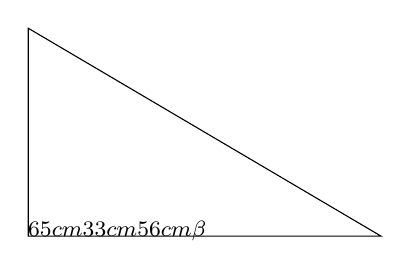
\begin{tikzpicture}[thin,scale=0.8]
				\coordinate (A) at (5.6,0);
				\coordinate (O) at (0,0);
				\coordinate (B) at (0,3.3);
				\draw (A)--(O)--(B)--cycle;
				\footnotesize
				\tkzLabelSegment[above=2pt,rotate=-atan(3.3/5.6)](B,A){$65\text{cm}$}
				\tkzLabelSegment[above=2pt,rotate=90](O,B){$33\text{cm}$}
				\tkzLabelSegment[below=2pt](O,A){$56\text{cm}$}
				\tkzMarkRightAngle[size=0.5](A,O,B)
				\tkzMarkAngle[size=1cm](O,B,A)
				\tkzLabelAngle[pos=0.6](O,B,A){$\beta$}
			\end{tikzpicture}
		\end{center}
		\columnbreak
		\begin{enumerate}
			\item $\csc(\beta)$
			\vspace{2cm}
			\item $\cot(\beta)$
			\vspace{2cm}
			\item $\cos(\beta)$
			\vspace{2cm}
		\end{enumerate}
	\end{multicols}
\end{myExit}
\vfill

\exitlikert{the \say{other} trigonometric functions}